%%%%%%%%%%%%%%%%%%%%%%%%%%%%%%%%%%%%%%%%%
% Short Sectioned Assignment
% LaTeX Template
% Version 1.0 (5/5/12)
%
% This template has been downloaded from:
% http://www.LaTeXTemplates.com
%
% Original author:
% Frits Wenneker (http://www.howtotex.com)
%
% License:
% CC BY-NC-SA 3.0 (http://creativecommons.org/licenses/by-nc-sa/3.0/)
%
%%%%%%%%%%%%%%%%%%%%%%%%%%%%%%%%%%%%%%%%%

%----------------------------------------------------------------------------------------
%	PACKAGES AND OTHER DOCUMENT CONFIGURATIONS
%----------------------------------------------------------------------------------------

\documentclass[paper=a4, fontsize=11pt]{article} % A4 paper and 11pt font size
\usepackage{geometry}
\geometry{left=1.8cm,right=1.8cm,top=1.2cm,bottom=2.5cm} % Magrin between the edge and content
\usepackage[T1]{fontenc} % Use 8-bit encoding that has 256 glyphs
\usepackage{fourier} % Use the Adobe Utopia font for the document - comment this line to return to the LaTeX default
\usepackage[english]{babel} % English language/hyphenation
\usepackage{amsmath,amsfonts,amsthm} % Math packages
\usepackage{graphicx} % Graph packages
\graphicspath{{../image/}}

\usepackage{lipsum} % Used for inserting dummy 'Lorem ipsum' text into the template

\usepackage{sectsty} % Allows customizing section commands
%\allsectionsfont{ \normalfont\scshape} % Make all sections centered, the default font and small caps
\usepackage{titlesec}
\titleformat*{\section}{\centering\Large\scshape}
\titleformat*{\subsection}{\large}

\usepackage{fancyhdr} % Custom headers and footers
\pagestyle{fancyplain} % Makes all pages in the document conform to the custom headers and footers
\fancyhead{} % No page header - if you want one, create it in the same way as the footers below
\fancyfoot[L]{} % Empty left footer
\fancyfoot[C]{\thepage} % Empty center footer
\fancyfoot[R]{} % Page numbering for right footer
\renewcommand{\headrulewidth}{0pt} % Remove header underlines
\renewcommand{\footrulewidth}{0pt} % Remove footer underlines
\setlength{\headheight}{13.6pt} % Customize the height of the header

\numberwithin{equation}{section} % Number equations within sections (i.e. 1.1, 1.2, 2.1, 2.2 instead of 1, 2, 3, 4)
\numberwithin{figure}{section} % Number figures within sections (i.e. 1.1, 1.2, 2.1, 2.2 instead of 1, 2, 3, 4)
\numberwithin{table}{section} % Number tables within sections (i.e. 1.1, 1.2, 2.1, 2.2 instead of 1, 2, 3, 4)

\setlength\parindent{0pt} % Removes all indentation from paragraphs - comment this line for an assignment with lots of text

%----------------------------------------------------------------------------------------
%	TITLE SECTION
%----------------------------------------------------------------------------------------

\newcommand{\horrule}[1]{\rule{\linewidth}{#1}} % Create horizontal rule command with 1 argument of height

\title{	
\normalfont \normalsize 
\textsc{
	Name: Yang Xiao	  \hfill 
	Student ID: 27748154	\hfill
	Email: yx5m14@soton.ac.uk \\ [25pt]} 
%\horrule{0.5pt} \\[0.4cm] % Thin top horizontal rule
\huge Computational Finance Assignment 1 (of 4) \\ % The assignment title
%\horrule{2pt} \\[0.5cm] % Thick bottom horizontal rule
}

%\author{Name: Yang Xiao} % Your name
\date{} % Today's date or a custom date

\begin{document}

\maketitle % Print the title

%----------------------------------------------------------------------------------------
%	EFFficient Frontier 
%----------------------------------------------------------------------------------------
\section{Efficient Frontier}

Assume that there are three stocks which follow Gaussian distribution with expected return \textbf{m},
\begin{align}
	m = [0.10\ 0.20\ 0.15]^{t}
\end{align}

and corresponding covariance \textbf{C},
\begin{align}
C = \begin{bmatrix}
0.005 & -0.010 & 0.004\\ 
-0.010 &  0.040& -0.002\\ 
0.004&  -0.002& 0.023
\end{bmatrix}
\end{align}


\subsection{Efficient Frontier and Random Portfolios}

Thus, in E-V space, the return of portfolios $r_{p}$
\begin{align}
r_{p}\sim \mathit{N}(\pi^{T}m, \pi^{T}C\pi)
\end{align}
where $\pi$ is a N$\times$1 vector of weights on N stocks subjected to $\sum_{i=1}^{N}\pi_{i}=1$.\\
By optimising the equation below, 
\begin{align}
\underset{\pi}{max}\ \pi^{T} m\ 
\end{align}

subject to $\pi^{T}C\pi=\sigma _{0}$

\begin{align}
\underset{\pi}{min}\  \pi^{T}C\pi\ 
\end{align}

subject to $\pi^{T} m = r_0$ \\

The optimal solutions can be attained.
\newpage
\textbf{Experiment: } The efficient frontier and 100 random portfolios can be drawn as the left figure in Figure 1.1. As can be seen, the random portfolios will never go above the efficient frontier. That is because the efficient frontier consists of the optimal solutions to the equation 1.4 and 1.5. 
By paring up stocks among these three stocks, from the right figure, we can learn that the random portfolios of these pair-up stocks only stay on the corresponding efficient frontier. And the random portfolios of three stocks can go below its efficient frontier. In addition, the efficient frontier of three stocks always stays above subsets' efficient frontiers and it seems like these pair-up efficient frontiers mark the boundary of all their parent portfolios. 
\begin{figure}[h!]
	\centering
	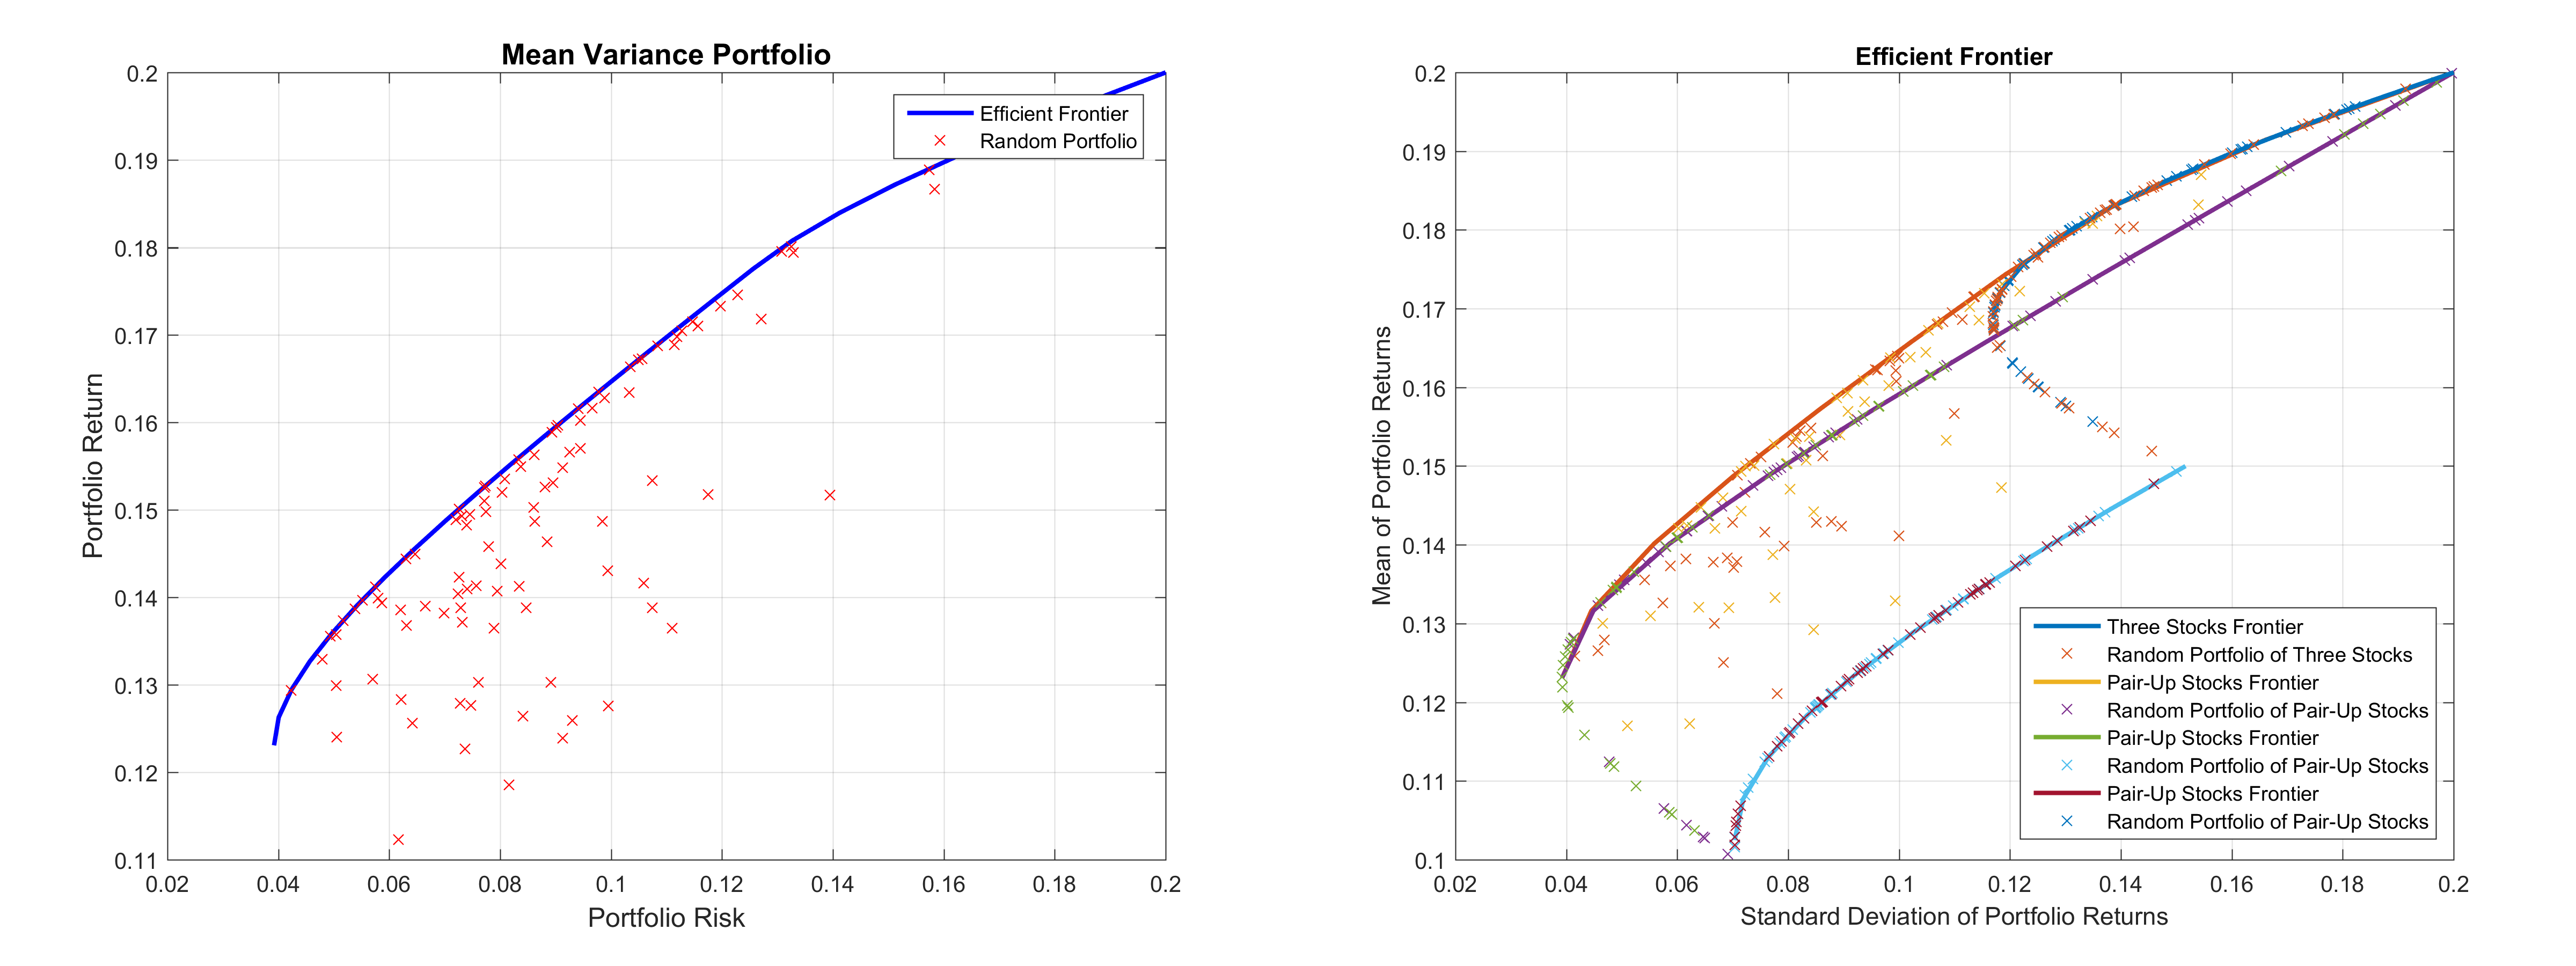
\includegraphics[width=18cm]{fig1_2.png}
	\caption{Mean Variance Portfolio}
\end{figure}

The boundary effect can be easier to notice by increasing the number of random portfolios to 10,000, which is shown in Figure 1.2.

\begin{figure}[h!]
	\centering
	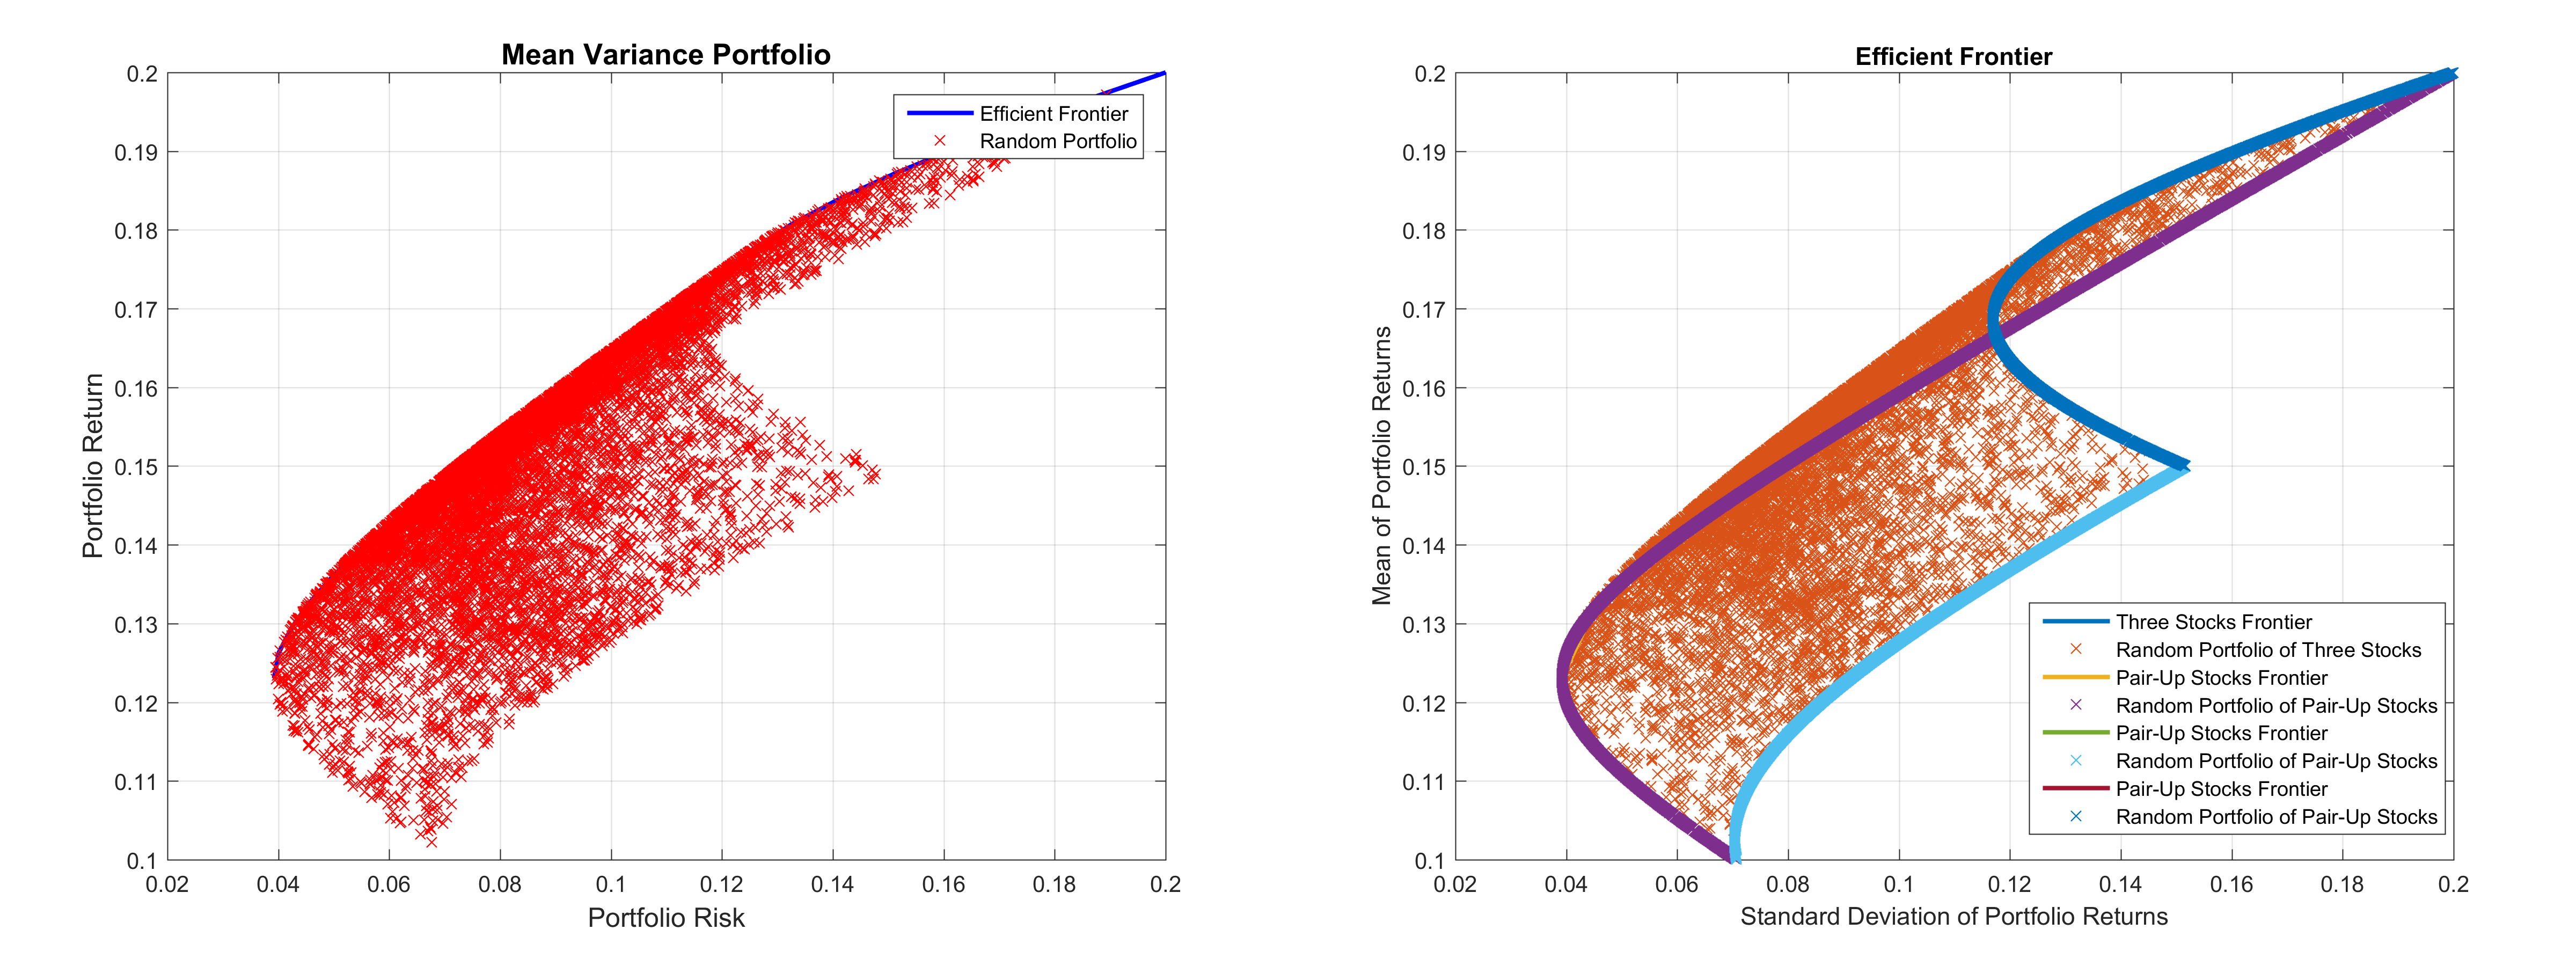
\includegraphics[width=18cm]{fig2_2.png}
	\caption{Mean Variance Portfolio with 10,000 random portfolios}
\end{figure}

To understand the underlying principle, we assume that expected return \textbf{m} of the pair-up child stocks is, 

\begin{align}
m = [m_1\ m_2]^{t}
\end{align}

and its corresponding covariance \textbf{C} is, 

\begin{align}
C = \begin{bmatrix}
\sigma_{1}^{2} & \sigma_{1}\sigma_{2}\\ 
\sigma_{1}\sigma_{2} & \sigma_{2}^{2}
\end{bmatrix}
\end{align}

The weight $\pi$ is, 
\begin{align}
m = [a\ b]^{t}
\end{align}
subject to $a+b=1$ \\

Therefore, we can write down the relationship between its corresponding portfolio risk, portfolio return and the weight of one stock. Here, take weight \textbf{a} as an example. 

\begin{align}
Risk =(a\ b)\begin{pmatrix}
\sigma_{1}^{2} & \sigma_{1}\sigma_{2}\\ 
\sigma_{1}\sigma_{2} & \sigma_{2}^{2}
\end{pmatrix}\binom{a}{b}=a^{2}\sigma _{1}^{2}+2ab\sigma _{1}\sigma _{2}+b^{2}\sigma _{2}^{2}
\end{align}

\begin{align}
Return = (a\ b)\binom{m_1}{m_2} = am_1 +bm_2
\end{align}

Simplify with $b=1-a$, then we have,
\begin{align}
Risk =(\sigma _{1}-\sigma _{2})^{2}a^{2}+2\sigma _{2}(\sigma _{1}-\sigma _{2})a+\sigma _{2}^{2}
\end{align}

\begin{align}
Return = (m_{1}-m_{2})a+m_{2}
\end{align}

From equation 1.11, we can know that the function of \textbf{Risk} and weight \textbf{a} is a curve. And the \textbf{Return} is a linear transform of \textbf{a}, which will not rotate the curve but only scale it. Considering all the information above, relationship between portfolio risk and weight and relationship between return and the risk can be drawn and shown as Figure 1.3.

\begin{figure}[h!]
	\centering
	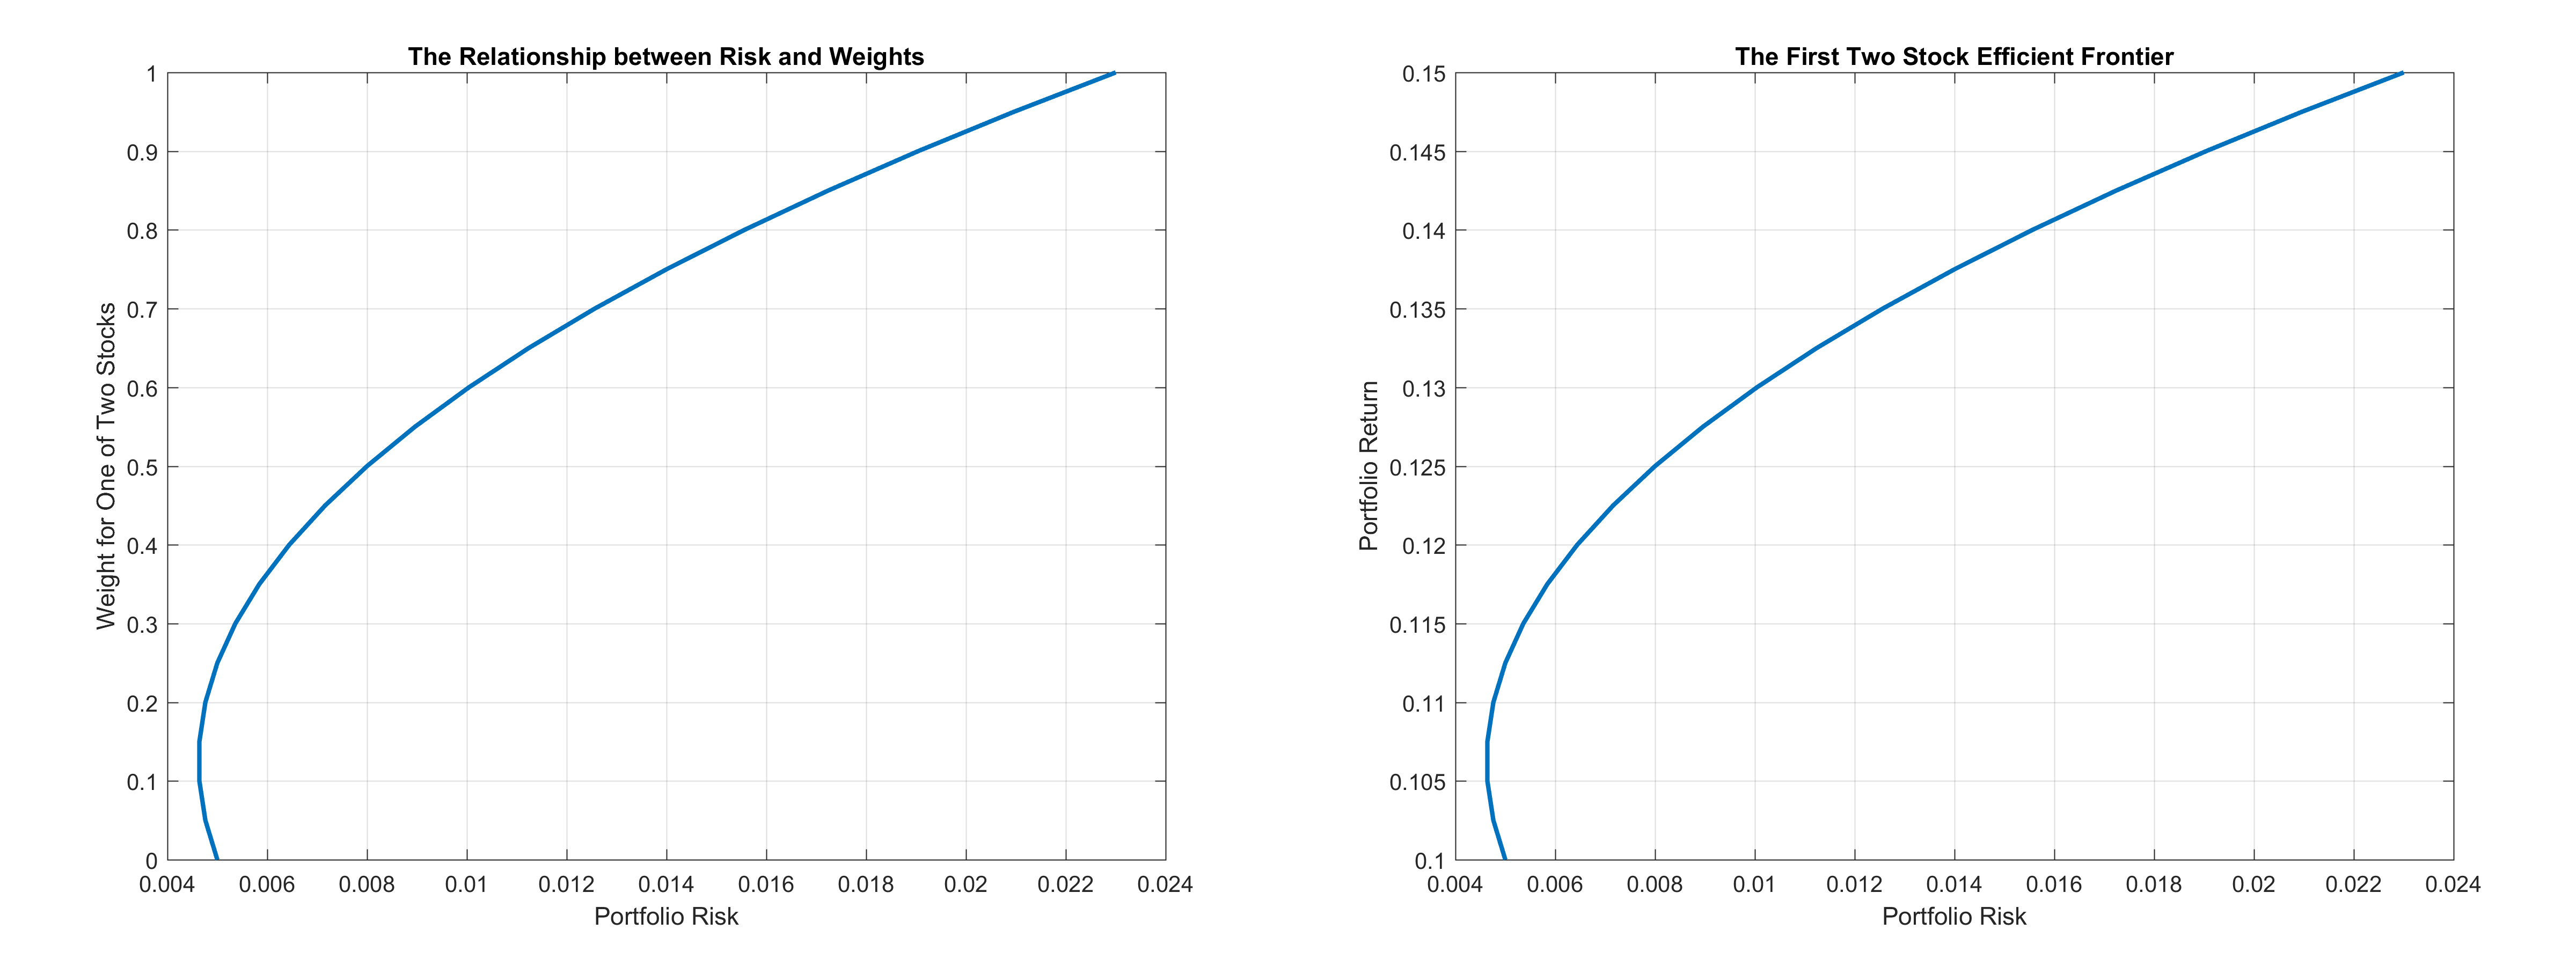
\includegraphics[width=18cm]{fig2_3.png}
	\caption{Relationship between Portfolio Risk and Weight and Relationship between Return and the risk}
\end{figure}

This figure makes more sense to the boundary effect. The reason of efficient frontier does not have the tail bit is that the \textbf{linprog} constraint decides that the starting point of the frontier will be the point with lowest risk, which is the bottom point of the quadratic curve. And the quadratic curve contains all the possible portfolios. That is why all the random portfolios stay on the curve. And this can also explain all the two-assets situations actually mark the boundary of their parent. 

\newpage
By replacing \textbf{linprog} and \textbf{quadprog} in the \textbf{NaiveMV} function with CVX tool, an identical result is expected. The result is shown as Figure 1.4.

\begin{figure}[h!]
	\centering
	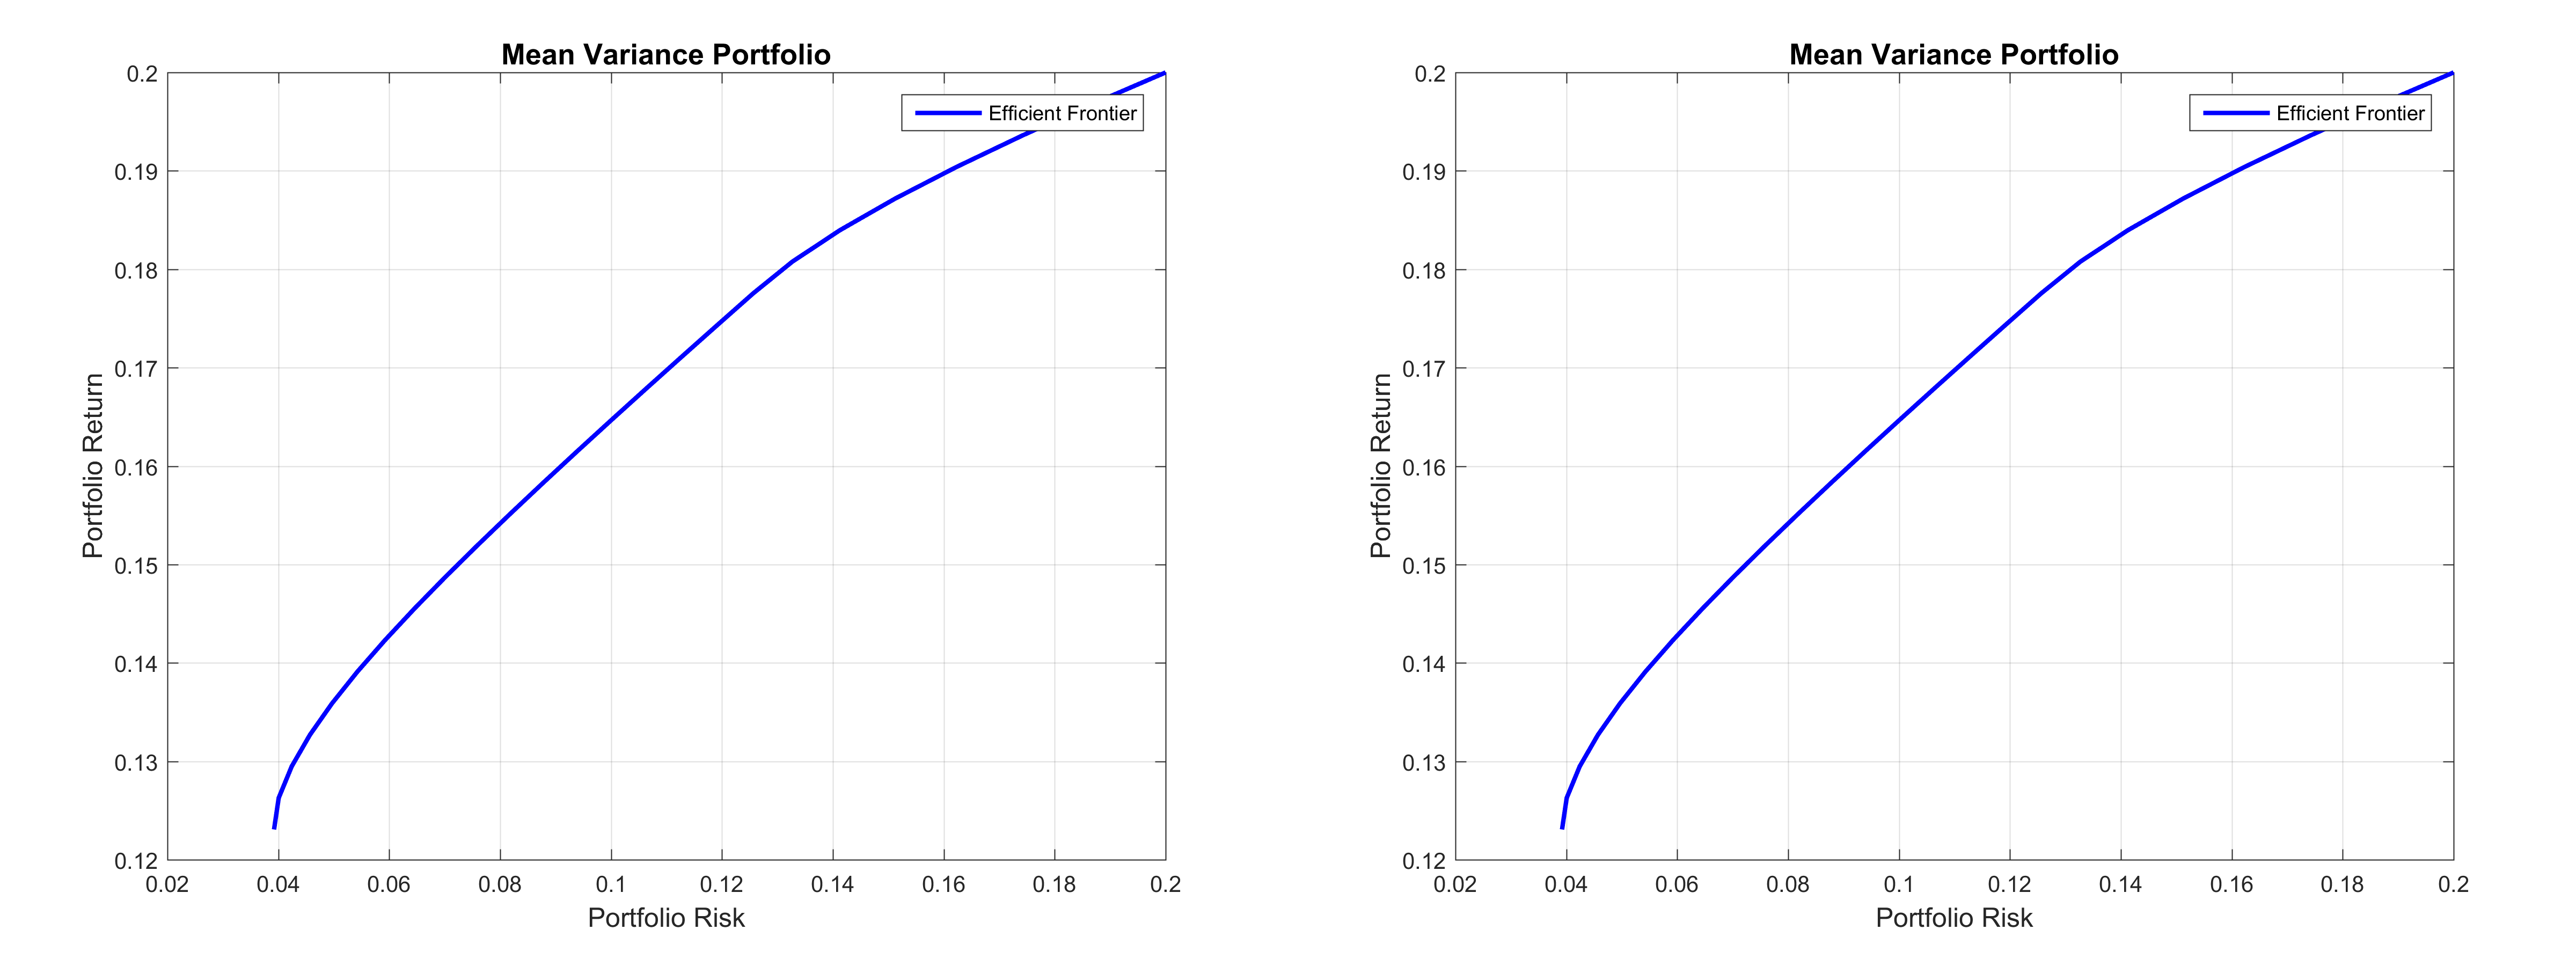
\includegraphics[width=18cm]{fig0_0.png}
	\caption{Mean Variance Portfolio by NaiveMV Function and by Altered NaiveMV Function}
\end{figure}

\section{Efficient Frontier on FTSE 100 Data}

\textbf{Data Preparation:} In this experiment, weekly data for the past 3 years is attained in order to avoid the inconvenience of imputing missing values of daily data. The size of the close price matrix is $217 \times 30$, which is a proper size of input. Next, calculate the weekly return rate with equation 2.1. 

\begin{align}
r=\frac{p_{n+1} - p_{n}}{p_{n}}
\end{align}
where \textit{p} is the close price of a stock and \textit{n} is the week. \\
After that, randomly select 3 stocks from $216 \times 30$ weekly return data and half them into a $108 \times 3 $ training subset and a $108 \times 3 $ testing subset. 

\subsection{Efficient Frontier and 1/N Portfolio on Training Data}
By using the method described in section 1, an efficient frontier of training data can be drawn as Figure 2.1. \\
For simple $1/N$ portfolio meaning that distributing the wealth into 3 stocks equally, thus, we can easily draw the situation onto the figure as well.

\newpage
\begin{figure}[h!]
	\centering
	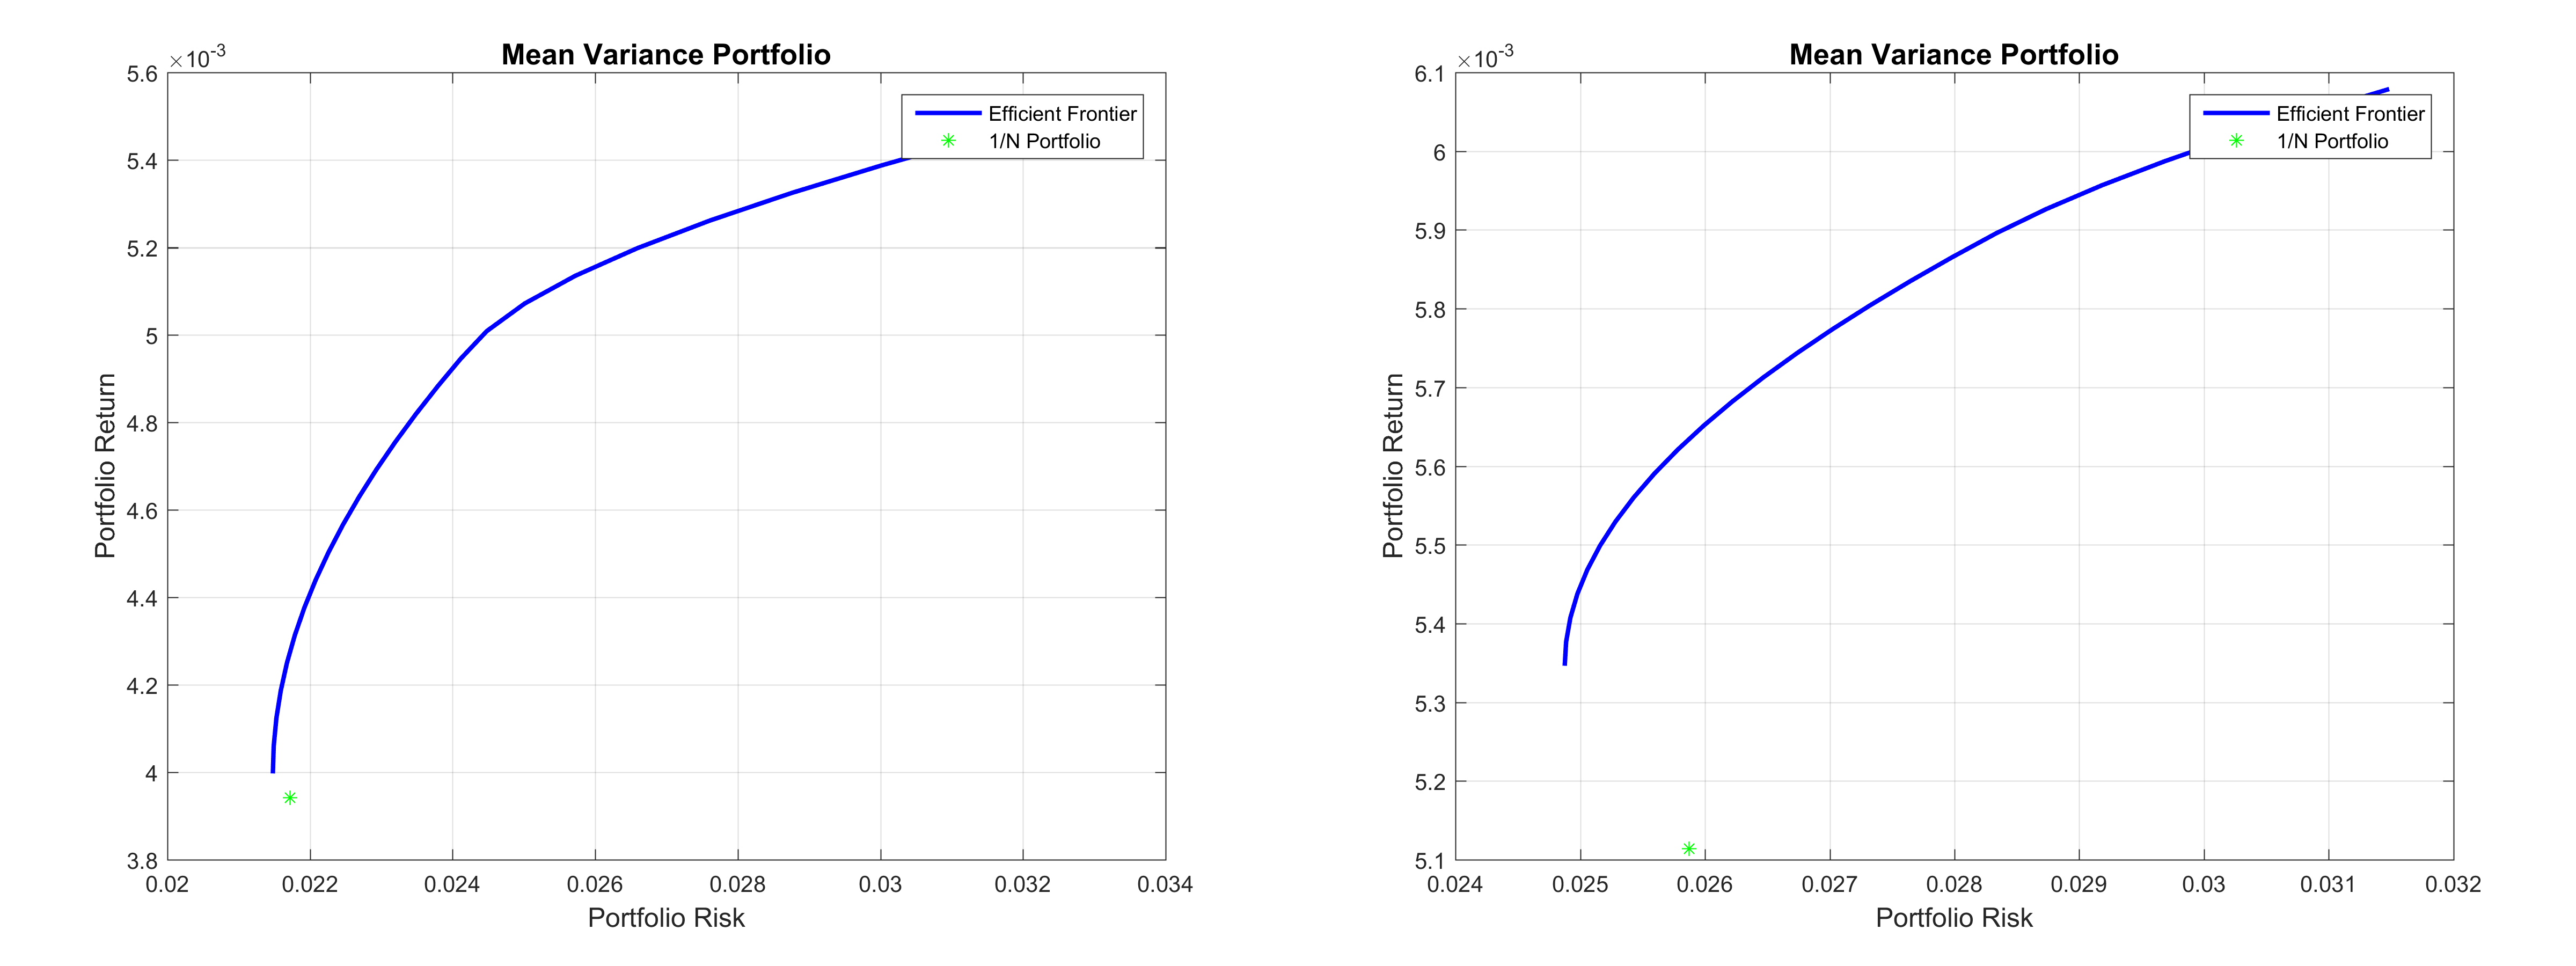
\includegraphics[width=18cm]{fig3_1.png}
	\caption{Efficient Frontier and 1/N Portfolio}
\end{figure}

As can be seen, simple $1/N$ portfolio will never be better than the portfolios on the efficient frontier since portfolios on the curve are the optimal on training data.

\subsection{Efficient Frontier and 1/N Portfolio on Testing Data}

Here, extract the corresponding weights of 25 points on the efficient frontier and conduct them on the testing data with equation 1.3. Then, the performance of these strategies can be shown on the Figure 2.2. 

\begin{figure}[h!]
	\centering
	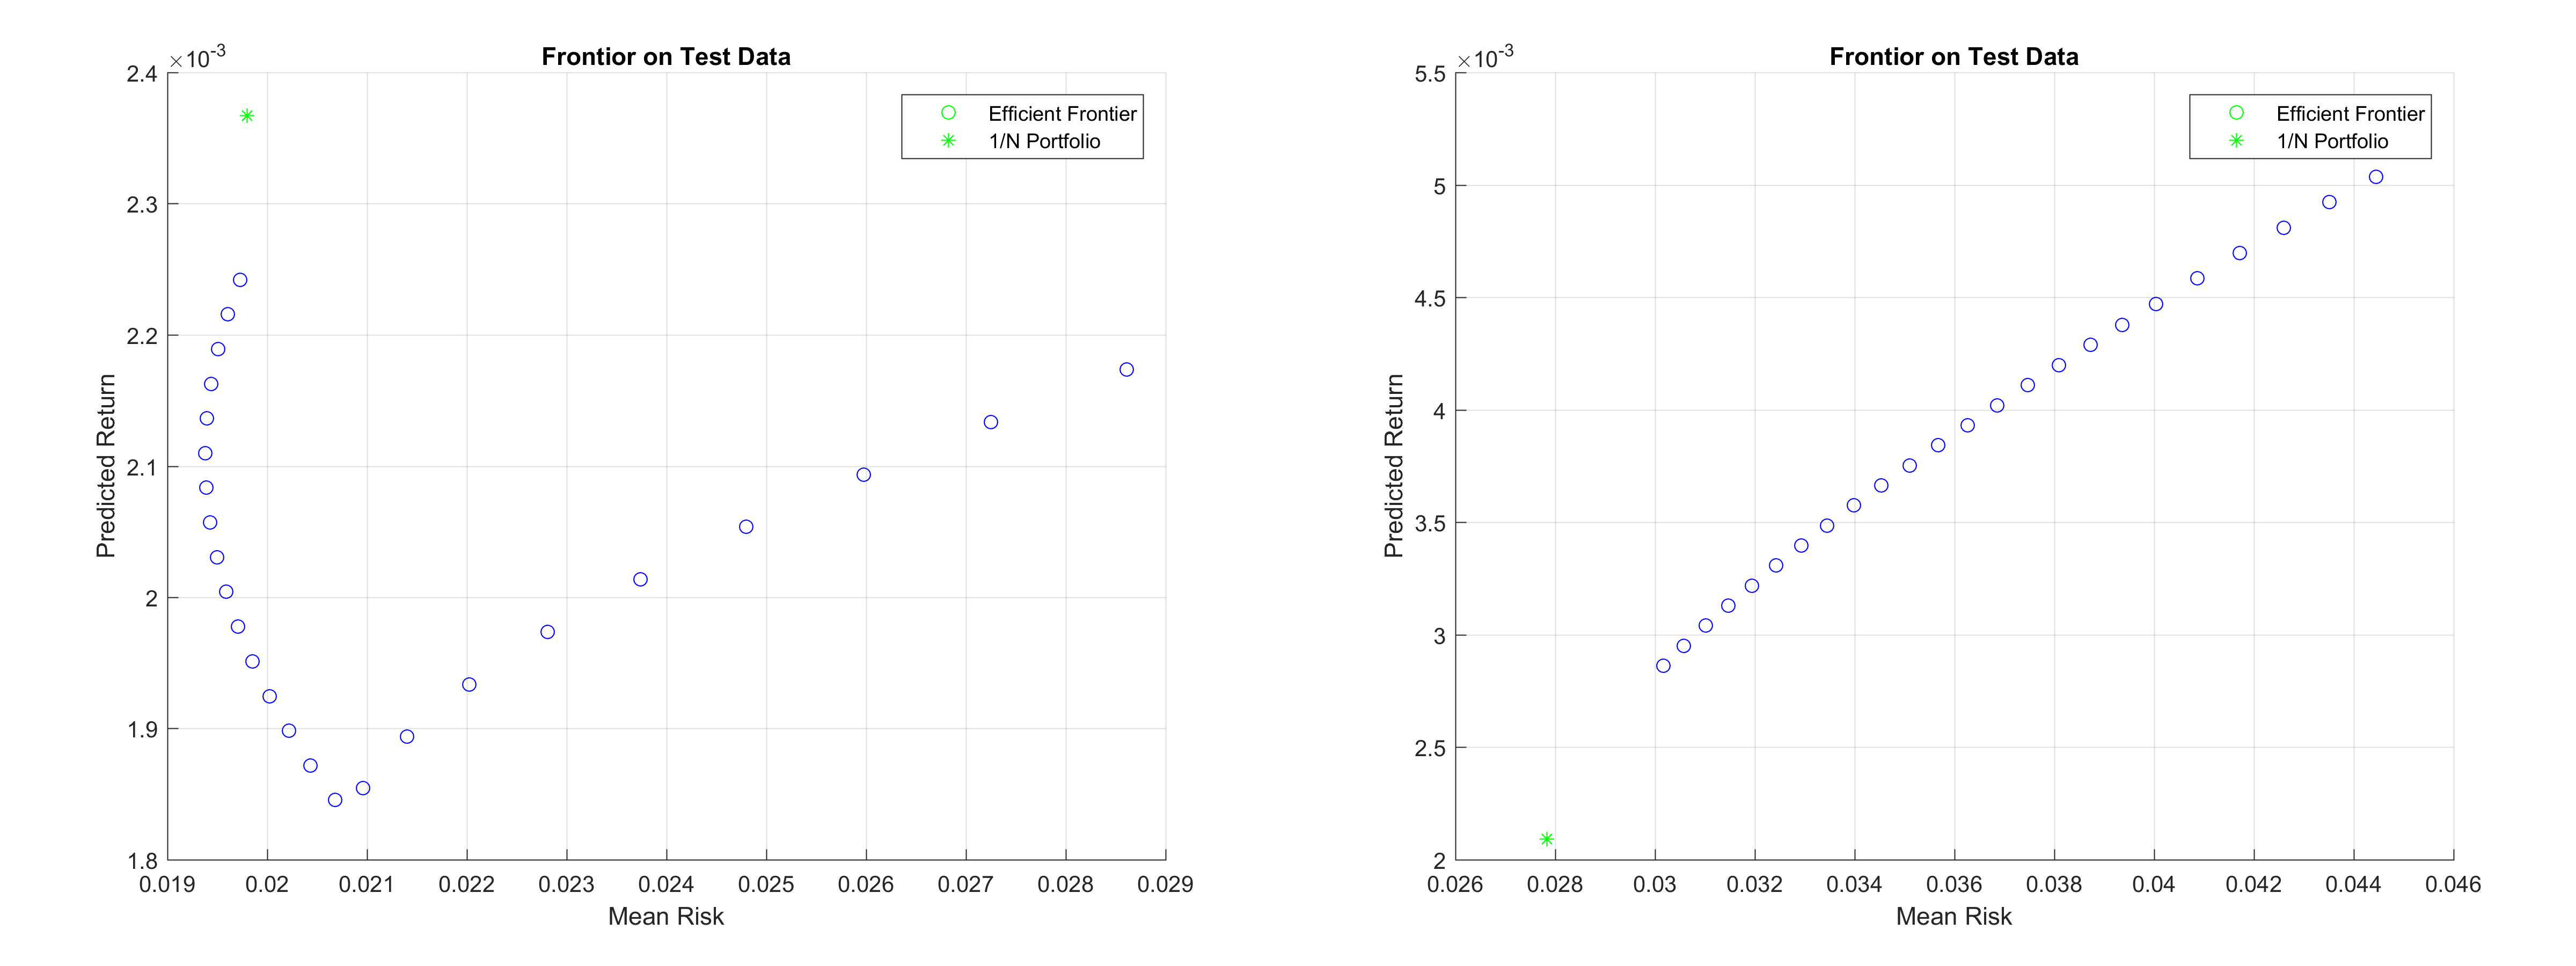
\includegraphics[width=18cm]{fig3_2.png}
	\caption{Efficient Frontier and 1/N Portfolio}
\end{figure}

As can be seen from the left figure, the performance of the $1/N$ portfolio on testing data is superior to those efficient portfolios attained from training subset. On the contrary, $1/N$ is worse on the performance on testing data than the efficient portfolios. In conclusion, the best strategies on training does not mean that they have the best performance on testing data. In other words, the anticipation from current data does not imply the future 100\% correctly. 

\section{Index Tracking}

Index tracking is for finding the stocks that have the same return as stock index. There are two strategies \textit{Greedy Selection} and \textit{Sparse Index Tracking} that will be discussed below.

\subsection{Greedy Forward Selection}

To find the stocks similar to \textit{FTSE Index}, we have to solve this equation,

\begin{align}
\underset{w}{min} \ ||y-Rw||_{2}^{2} \ subject\ to\ ||w||_{0} = w_{0}
\end{align}
where \textit{y} is the \textit{FTSE Index}, \textit{R} is the return rate data above, \textit{w} is the corresponding weight and $w_0$ is the number of selection stocks. 

Thus, 6 stocks can be found and listed below. 

\begin{table}[h!]
	\centering
	\begin{tabular}{|c|c|c|c|c|c|c|}
		\hline
		Indices &  15 &  20 & 8 & 6 & 9 & 21 \\ 
		\hline
		Stocks' Name & BKG.L & BRBY.L & AV.L & ANTO.L & AZN.L & BT-A.L \\
		\hline
	\end{tabular}
	\caption{The Six Stocks Most Similar to FTSE Index}
\end{table}

\subsection{Sparse Index Tracking}

\begin{align}
\underset{w}{min} \ [||y-Rw||_{2}^{2}-\tau ||w||_{1}]
\end{align}

By ranging the $\tau$ from 0.01 to 0.7, the figure that implies the relationship between $\tau$ and the  number of non-zero weights can be drawn and shown as Figure 3.1.

\begin{figure}[h!]
	\centering
	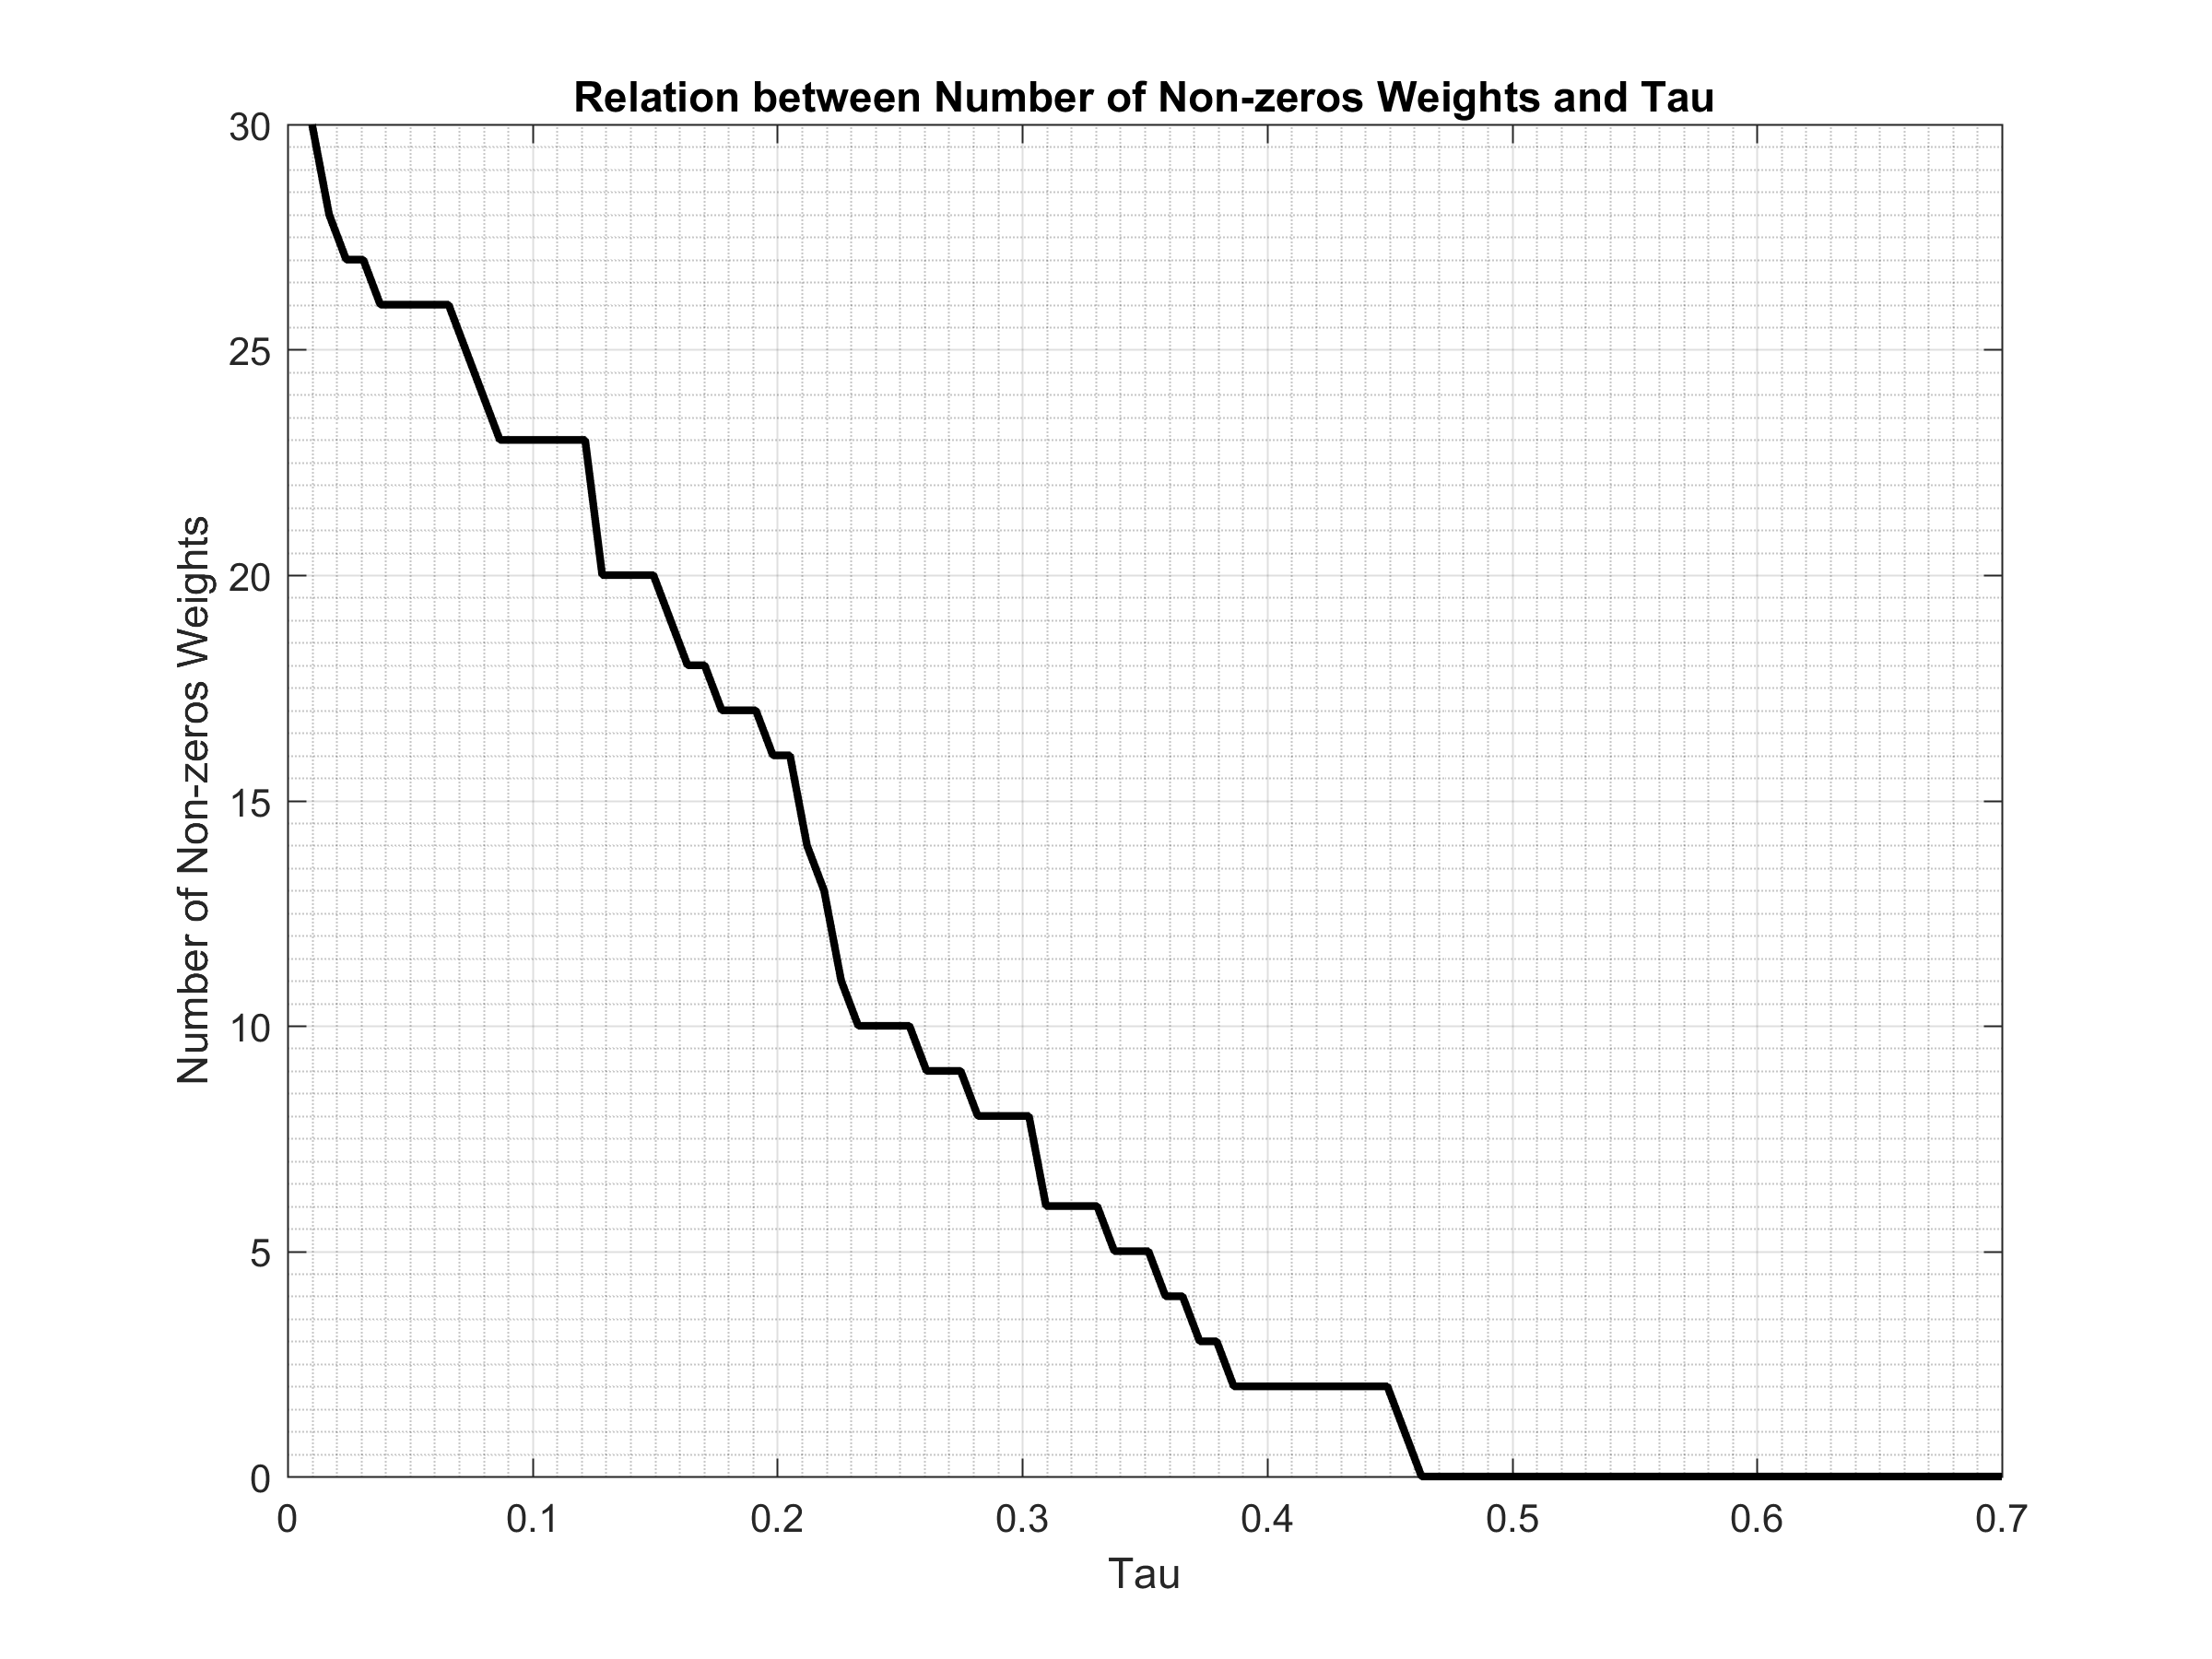
\includegraphics[width=9cm]{fig6.png}
	\caption{Relation between Number of Non-zeros Weights and Tau}
\end{figure}

As can be seen from the figure, we can get six specific stocks when taking $\tau$ as a value among 0.31 to 0.34. 

\begin{table}[h!]
	\centering
	\begin{tabular}{|c|c|c|c|c|c|c|}
		\hline
		Indices &  25 &  29 & 1 & 3 & 7 & 17 \\ 
		\hline
		Stocks' Name & CPG.L & EXPN.L & AAL.L & ADM.L & ARM.L & BLT.L \\
		\hline
	\end{tabular}
	\caption{The Six Stocks Most Similar to FTSE Index by Sparse Index Tracking}
\end{table}


\newpage
\section{Portfolio Optimisation with Transaction Costs}

According to the research from \textit{Lobo et al.} in 2007, portfolio optimisation with transaction costs problem can be narrowed down to optimise the equations listed below. 

\begin{align}
maximise\ a^{T}(w+x^{+}-x^{-})
\end{align}
subject to
\begin{align}
&1^{T}(x^{+}-x^{-})+\sum_{i=1}^{n}(a_{i}^{+}x_{i}^{+}+a_{i}^{-}x_{i}^{-}) \leqslant 0\\
&x^{+}\geqslant 0,\ x^{-}\geqslant 0,\ i=1,2,\cdots n\\
&w_{i}+x_{i}^{+}-x_{i}^{-}\geqslant S_{i}, \ i=1,2,\cdots n\\
&\phi ^{-1}(\eta _{i})||C^{\frac{1}{2}}(w+x^{+}-x^{-})||\leqslant a^{T}(w+x^{+}-x^{-})-W_{j}^{low}, \ j=1,2
\end{align}

where $x^{+}$ and $x^{-}$ are the buying and selling adjustment weight on stocks respectively. $a^{T}$ is the expected return, and $w$ is the weight vector on invested stocks.\\ 
\textbf{Budget Constraint: } constraint 4.2 states that after adjusting the weights on stocks, the change in current wealth is $\mathit{1^{T}(x^{+}-x^{-})}$. And the sum of wealth change and transaction fees $\mathit{a_{i}^{+}x_{i}^{+}+a_{i}^{-}x_{i}^{-}}$should not be less than 0. Otherwise, this adjustment would not be a wise choice since you would lose money by doing this adjustment.\\
\textbf{Shortselling Constraint: } this constraint is shown by equation 4.4 meaning that the adjustment on stocks have individual limit. For example, if shortselling on some stocks is not allowed, the adjustment $\mathit{w_{i}+x_{i}^{+}-x_{i}^{-}}$ on these stocks must be positive. Similarly, if shortselling is permitted, $S_{i}$ is dependent on the amount of weights of shortselling allowed.\\
\textbf{Shortfall Risk Constraint: } this constraint 4.5 comes from the the equation $Prob(W\leqslant  W^{low})\leqslant 1-\eta $, which means that how much possibility that I will get a wealth lower than than my expectation for the lowest return $W^{low}$. Under the assumption that expected return $W$ follows Gaussian distribution, we can simply the equation into constraint 4.5.\\



%----------------------------------------------------------------------------------------

\end{document}